\documentclass[14pt,letterpaper]{extarticle}
\usepackage[T1]{fontenc}
\usepackage{tgheros}
\renewcommand{\familydefault}{\sfdefault}
\usepackage[letterpaper, left=0.75in, right=0.75in, top=0.85in, bottom=0.85in,
  headheight=16pt, headsep=14pt, footskip=26pt]{geometry}
\usepackage{fancyhdr}
\usepackage{pifont}
\usepackage{tikz}
\usetikzlibrary{arrows.meta}
\pagestyle{fancy}
\fancyhf{}
\fancyhead[L]{Week NN / Train-yard sorting / Grades K–1}
\fancyfoot[L]{\small Bellingham Math Circle / Week NN / TY-K-v1}
\fancyfoot[R]{\small \thepage}
\renewcommand{\headrulewidth}{0.4pt}
\renewcommand{\footrulewidth}{0pt}
\setlength{\parindent}{0pt}
\setlength{\parskip}{4pt}
\newcommand{\problem}[1]{\par\vspace{14pt}\noindent\textbf{Problem #1:} }
\newcommand{\yes}{\ding{51}}
\newcommand{\no}{\ding{55}}
\begin{document}

Line up a train on the arrival track the way it is drawn. The car on the left goes first, and cars never jump over each other. Each car drives down into the siding and then out to the departure track. Only the top car in the siding can drive out. Car 1 must leave first, then car 2, then car 3, and so on.

\par\vspace{2pt}\begin{center}
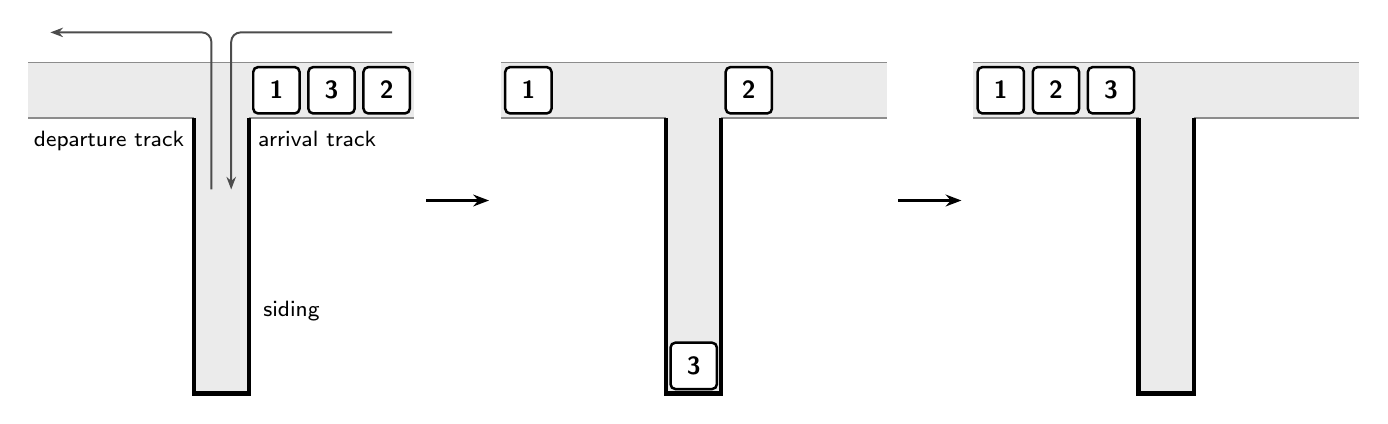
\begin{tikzpicture}[x=1mm,y=1mm]
\begin{scope}[shift={(21,0)}]
\fill[black!8] (-21,0) rectangle (28,7);
\fill[black!8] (0,-35) rectangle (7,0);
\draw[black!45, line width=0.5pt] (-21,7) -- (28,7);
\draw[black!45, line width=0.5pt] (-21,0) -- (0,0);
\draw[black!45, line width=0.5pt] (7,0) -- (28,0);
\draw[line width=1.6pt] (0,0) -- (0,-35) -- (7,-35) -- (7,0);
\draw[line width=0.9pt, fill=white, rounded corners=0.6mm] (7.56,0.56) rectangle (13.44,6.44);
\node at (10.5,3.5) {\bfseries\small 1};
\draw[line width=0.9pt, fill=white, rounded corners=0.6mm] (14.56,0.56) rectangle (20.44,6.44);
\node at (17.5,3.5) {\bfseries\small 3};
\draw[line width=0.9pt, fill=white, rounded corners=0.6mm] (21.56,0.56) rectangle (27.44,6.44);
\node at (24.5,3.5) {\bfseries\small 2};
\node[font=\footnotesize, below left, inner xsep=1pt] at (-0.8,-0.4) {departure track};
\node[font=\footnotesize, below right, inner xsep=1pt] at (7.8,-0.4) {arrival track};
\node[font=\footnotesize, right] at (7.6,-24.5) {siding};
\draw[-{Stealth[length=1.6mm]}, line width=0.7pt, black!70, rounded corners=1.2mm] (25.2,10.85) -- (4.76,10.85) -- (4.76,-9.1);
\draw[-{Stealth[length=1.6mm]}, line width=0.7pt, black!70, rounded corners=1.2mm] (2.24,-9.1) -- (2.24,10.85) -- (-18.2,10.85);
\end{scope}
\draw[-{Stealth[length=2mm]}, line width=0.9pt] (50.5,-10.5) -- (58.5,-10.5);
\begin{scope}[shift={(81,0)}]
\fill[black!8] (-21,0) rectangle (28,7);
\fill[black!8] (0,-35) rectangle (7,0);
\draw[black!45, line width=0.5pt] (-21,7) -- (28,7);
\draw[black!45, line width=0.5pt] (-21,0) -- (0,0);
\draw[black!45, line width=0.5pt] (7,0) -- (28,0);
\draw[line width=1.6pt] (0,0) -- (0,-35) -- (7,-35) -- (7,0);
\draw[line width=0.9pt, fill=white, rounded corners=0.6mm] (-20.44,0.56) rectangle (-14.56,6.44);
\node at (-17.5,3.5) {\bfseries\small 1};
\draw[line width=0.9pt, fill=white, rounded corners=0.6mm] (0.56,-34.44) rectangle (6.44,-28.56);
\node at (3.5,-31.5) {\bfseries\small 3};
\draw[line width=0.9pt, fill=white, rounded corners=0.6mm] (7.56,0.56) rectangle (13.44,6.44);
\node at (10.5,3.5) {\bfseries\small 2};
\end{scope}
\draw[-{Stealth[length=2mm]}, line width=0.9pt] (110.5,-10.5) -- (118.5,-10.5);
\begin{scope}[shift={(141,0)}]
\fill[black!8] (-21,0) rectangle (28,7);
\fill[black!8] (0,-35) rectangle (7,0);
\draw[black!45, line width=0.5pt] (-21,7) -- (28,7);
\draw[black!45, line width=0.5pt] (-21,0) -- (0,0);
\draw[black!45, line width=0.5pt] (7,0) -- (28,0);
\draw[line width=1.6pt] (0,0) -- (0,-35) -- (7,-35) -- (7,0);
\draw[line width=0.9pt, fill=white, rounded corners=0.6mm] (-20.44,0.56) rectangle (-14.56,6.44);
\node at (-17.5,3.5) {\bfseries\small 1};
\draw[line width=0.9pt, fill=white, rounded corners=0.6mm] (-13.44,0.56) rectangle (-7.56,6.44);
\node at (-10.5,3.5) {\bfseries\small 2};
\draw[line width=0.9pt, fill=white, rounded corners=0.6mm] (-6.44,0.56) rectangle (-0.56,6.44);
\node at (-3.5,3.5) {\bfseries\small 3};
\end{scope}
\end{tikzpicture}
\end{center}

\problem{1}Which of these trains can leave 1, 2, 3? Mark each one \yes{} or \no, and show with the cars why each \no{} train gets stuck.
\par\vspace{8pt}\begin{center}
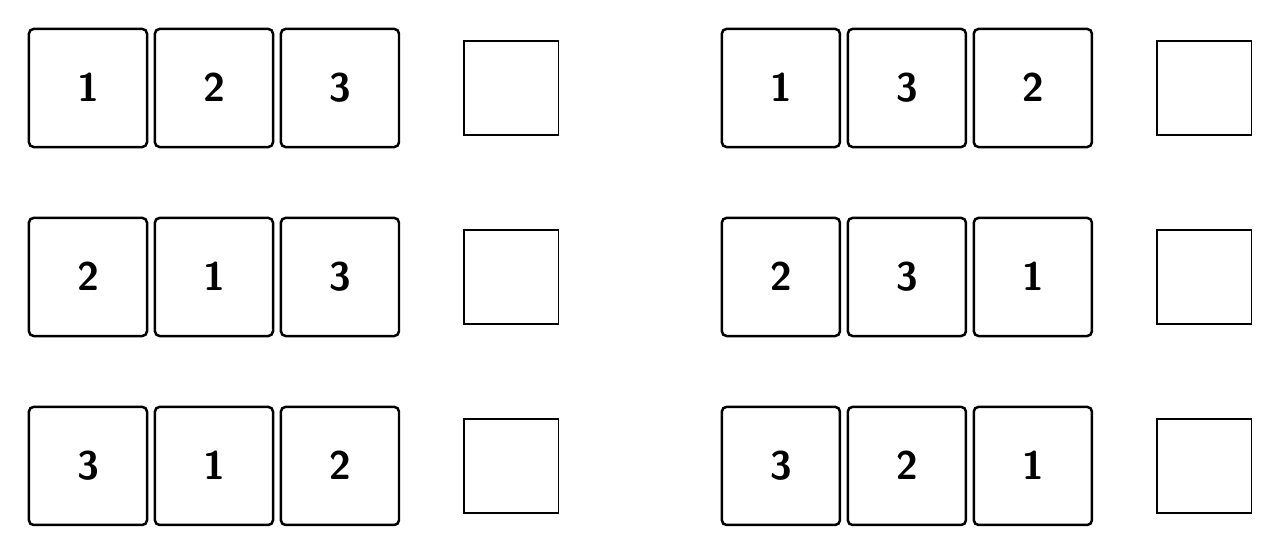
\begin{tikzpicture}[x=1mm,y=1mm]
\draw[line width=0.9pt, fill=white, rounded corners=0.6mm] (0,0) rectangle (15,15);
\node at (7.5,7.5) {\bfseries\Large 1};
\draw[line width=0.9pt, fill=white, rounded corners=0.6mm] (16,0) rectangle (31,15);
\node at (23.5,7.5) {\bfseries\Large 2};
\draw[line width=0.9pt, fill=white, rounded corners=0.6mm] (32,0) rectangle (47,15);
\node at (39.5,7.5) {\bfseries\Large 3};
\draw[line width=0.6pt] (55.25,1.5) rectangle (67.25,13.5);
\draw[line width=0.9pt, fill=white, rounded corners=0.6mm] (88,0) rectangle (103,15);
\node at (95.5,7.5) {\bfseries\Large 1};
\draw[line width=0.9pt, fill=white, rounded corners=0.6mm] (104,0) rectangle (119,15);
\node at (111.5,7.5) {\bfseries\Large 3};
\draw[line width=0.9pt, fill=white, rounded corners=0.6mm] (120,0) rectangle (135,15);
\node at (127.5,7.5) {\bfseries\Large 2};
\draw[line width=0.6pt] (143.25,1.5) rectangle (155.25,13.5);
\draw[line width=0.9pt, fill=white, rounded corners=0.6mm] (0,-24) rectangle (15,-9);
\node at (7.5,-16.5) {\bfseries\Large 2};
\draw[line width=0.9pt, fill=white, rounded corners=0.6mm] (16,-24) rectangle (31,-9);
\node at (23.5,-16.5) {\bfseries\Large 1};
\draw[line width=0.9pt, fill=white, rounded corners=0.6mm] (32,-24) rectangle (47,-9);
\node at (39.5,-16.5) {\bfseries\Large 3};
\draw[line width=0.6pt] (55.25,-22.5) rectangle (67.25,-10.5);
\draw[line width=0.9pt, fill=white, rounded corners=0.6mm] (88,-24) rectangle (103,-9);
\node at (95.5,-16.5) {\bfseries\Large 2};
\draw[line width=0.9pt, fill=white, rounded corners=0.6mm] (104,-24) rectangle (119,-9);
\node at (111.5,-16.5) {\bfseries\Large 3};
\draw[line width=0.9pt, fill=white, rounded corners=0.6mm] (120,-24) rectangle (135,-9);
\node at (127.5,-16.5) {\bfseries\Large 1};
\draw[line width=0.6pt] (143.25,-22.5) rectangle (155.25,-10.5);
\draw[line width=0.9pt, fill=white, rounded corners=0.6mm] (0,-48) rectangle (15,-33);
\node at (7.5,-40.5) {\bfseries\Large 3};
\draw[line width=0.9pt, fill=white, rounded corners=0.6mm] (16,-48) rectangle (31,-33);
\node at (23.5,-40.5) {\bfseries\Large 1};
\draw[line width=0.9pt, fill=white, rounded corners=0.6mm] (32,-48) rectangle (47,-33);
\node at (39.5,-40.5) {\bfseries\Large 2};
\draw[line width=0.6pt] (55.25,-46.5) rectangle (67.25,-34.5);
\draw[line width=0.9pt, fill=white, rounded corners=0.6mm] (88,-48) rectangle (103,-33);
\node at (95.5,-40.5) {\bfseries\Large 3};
\draw[line width=0.9pt, fill=white, rounded corners=0.6mm] (104,-48) rectangle (119,-33);
\node at (111.5,-40.5) {\bfseries\Large 2};
\draw[line width=0.9pt, fill=white, rounded corners=0.6mm] (120,-48) rectangle (135,-33);
\node at (127.5,-40.5) {\bfseries\Large 1};
\draw[line width=0.6pt] (143.25,-46.5) rectangle (155.25,-34.5);
\end{tikzpicture}
\end{center}

\newpage
\problem{2}Which of these trains can leave 1, 2, 3, 4? Mark each one \yes{} or \no.
\par\vspace{8pt}\begin{center}
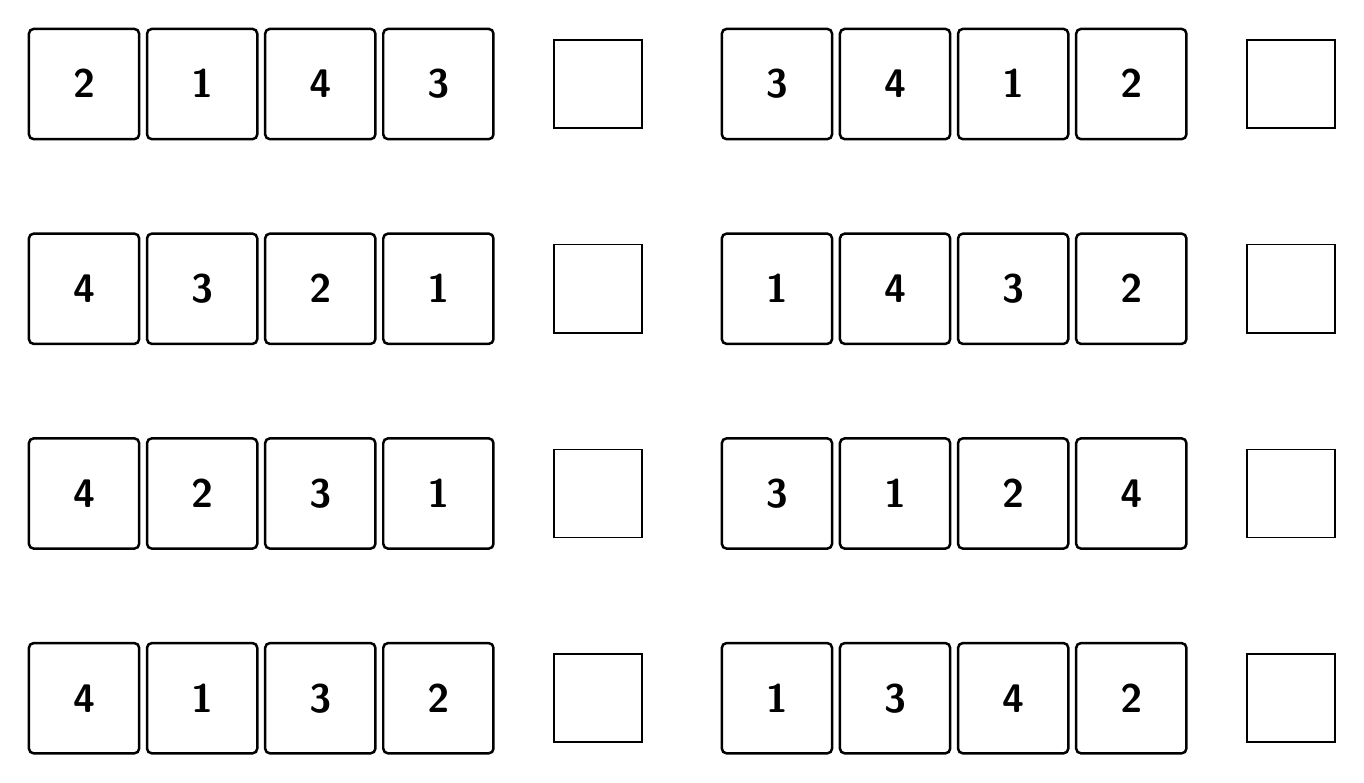
\begin{tikzpicture}[x=1mm,y=1mm]
\draw[line width=0.9pt, fill=white, rounded corners=0.6mm] (0,0) rectangle (14,14);
\node at (7,7) {\bfseries\Large 2};
\draw[line width=0.9pt, fill=white, rounded corners=0.6mm] (15,0) rectangle (29,14);
\node at (22,7) {\bfseries\Large 1};
\draw[line width=0.9pt, fill=white, rounded corners=0.6mm] (30,0) rectangle (44,14);
\node at (37,7) {\bfseries\Large 4};
\draw[line width=0.9pt, fill=white, rounded corners=0.6mm] (45,0) rectangle (59,14);
\node at (52,7) {\bfseries\Large 3};
\draw[line width=0.6pt] (66.7,1.4) rectangle (77.9,12.6);
\draw[line width=0.9pt, fill=white, rounded corners=0.6mm] (88,0) rectangle (102,14);
\node at (95,7) {\bfseries\Large 3};
\draw[line width=0.9pt, fill=white, rounded corners=0.6mm] (103,0) rectangle (117,14);
\node at (110,7) {\bfseries\Large 4};
\draw[line width=0.9pt, fill=white, rounded corners=0.6mm] (118,0) rectangle (132,14);
\node at (125,7) {\bfseries\Large 1};
\draw[line width=0.9pt, fill=white, rounded corners=0.6mm] (133,0) rectangle (147,14);
\node at (140,7) {\bfseries\Large 2};
\draw[line width=0.6pt] (154.7,1.4) rectangle (165.9,12.6);
\draw[line width=0.9pt, fill=white, rounded corners=0.6mm] (0,-26) rectangle (14,-12);
\node at (7,-19) {\bfseries\Large 4};
\draw[line width=0.9pt, fill=white, rounded corners=0.6mm] (15,-26) rectangle (29,-12);
\node at (22,-19) {\bfseries\Large 3};
\draw[line width=0.9pt, fill=white, rounded corners=0.6mm] (30,-26) rectangle (44,-12);
\node at (37,-19) {\bfseries\Large 2};
\draw[line width=0.9pt, fill=white, rounded corners=0.6mm] (45,-26) rectangle (59,-12);
\node at (52,-19) {\bfseries\Large 1};
\draw[line width=0.6pt] (66.7,-24.6) rectangle (77.9,-13.4);
\draw[line width=0.9pt, fill=white, rounded corners=0.6mm] (88,-26) rectangle (102,-12);
\node at (95,-19) {\bfseries\Large 1};
\draw[line width=0.9pt, fill=white, rounded corners=0.6mm] (103,-26) rectangle (117,-12);
\node at (110,-19) {\bfseries\Large 4};
\draw[line width=0.9pt, fill=white, rounded corners=0.6mm] (118,-26) rectangle (132,-12);
\node at (125,-19) {\bfseries\Large 3};
\draw[line width=0.9pt, fill=white, rounded corners=0.6mm] (133,-26) rectangle (147,-12);
\node at (140,-19) {\bfseries\Large 2};
\draw[line width=0.6pt] (154.7,-24.6) rectangle (165.9,-13.4);
\draw[line width=0.9pt, fill=white, rounded corners=0.6mm] (0,-52) rectangle (14,-38);
\node at (7,-45) {\bfseries\Large 4};
\draw[line width=0.9pt, fill=white, rounded corners=0.6mm] (15,-52) rectangle (29,-38);
\node at (22,-45) {\bfseries\Large 2};
\draw[line width=0.9pt, fill=white, rounded corners=0.6mm] (30,-52) rectangle (44,-38);
\node at (37,-45) {\bfseries\Large 3};
\draw[line width=0.9pt, fill=white, rounded corners=0.6mm] (45,-52) rectangle (59,-38);
\node at (52,-45) {\bfseries\Large 1};
\draw[line width=0.6pt] (66.7,-50.6) rectangle (77.9,-39.4);
\draw[line width=0.9pt, fill=white, rounded corners=0.6mm] (88,-52) rectangle (102,-38);
\node at (95,-45) {\bfseries\Large 3};
\draw[line width=0.9pt, fill=white, rounded corners=0.6mm] (103,-52) rectangle (117,-38);
\node at (110,-45) {\bfseries\Large 1};
\draw[line width=0.9pt, fill=white, rounded corners=0.6mm] (118,-52) rectangle (132,-38);
\node at (125,-45) {\bfseries\Large 2};
\draw[line width=0.9pt, fill=white, rounded corners=0.6mm] (133,-52) rectangle (147,-38);
\node at (140,-45) {\bfseries\Large 4};
\draw[line width=0.6pt] (154.7,-50.6) rectangle (165.9,-39.4);
\draw[line width=0.9pt, fill=white, rounded corners=0.6mm] (0,-78) rectangle (14,-64);
\node at (7,-71) {\bfseries\Large 4};
\draw[line width=0.9pt, fill=white, rounded corners=0.6mm] (15,-78) rectangle (29,-64);
\node at (22,-71) {\bfseries\Large 1};
\draw[line width=0.9pt, fill=white, rounded corners=0.6mm] (30,-78) rectangle (44,-64);
\node at (37,-71) {\bfseries\Large 3};
\draw[line width=0.9pt, fill=white, rounded corners=0.6mm] (45,-78) rectangle (59,-64);
\node at (52,-71) {\bfseries\Large 2};
\draw[line width=0.6pt] (66.7,-76.6) rectangle (77.9,-65.4);
\draw[line width=0.9pt, fill=white, rounded corners=0.6mm] (88,-78) rectangle (102,-64);
\node at (95,-71) {\bfseries\Large 1};
\draw[line width=0.9pt, fill=white, rounded corners=0.6mm] (103,-78) rectangle (117,-64);
\node at (110,-71) {\bfseries\Large 3};
\draw[line width=0.9pt, fill=white, rounded corners=0.6mm] (118,-78) rectangle (132,-64);
\node at (125,-71) {\bfseries\Large 4};
\draw[line width=0.9pt, fill=white, rounded corners=0.6mm] (133,-78) rectangle (147,-64);
\node at (140,-71) {\bfseries\Large 2};
\draw[line width=0.6pt] (154.7,-76.6) rectangle (165.9,-65.4);
\end{tikzpicture}
\end{center}

\newpage
\problem{3}Car 1 is last in each of these trains. Fill in cars 2, 3, 4 in different ways, and find every train that can leave 1, 2, 3, 4.
\par\vspace{8pt}\begin{center}
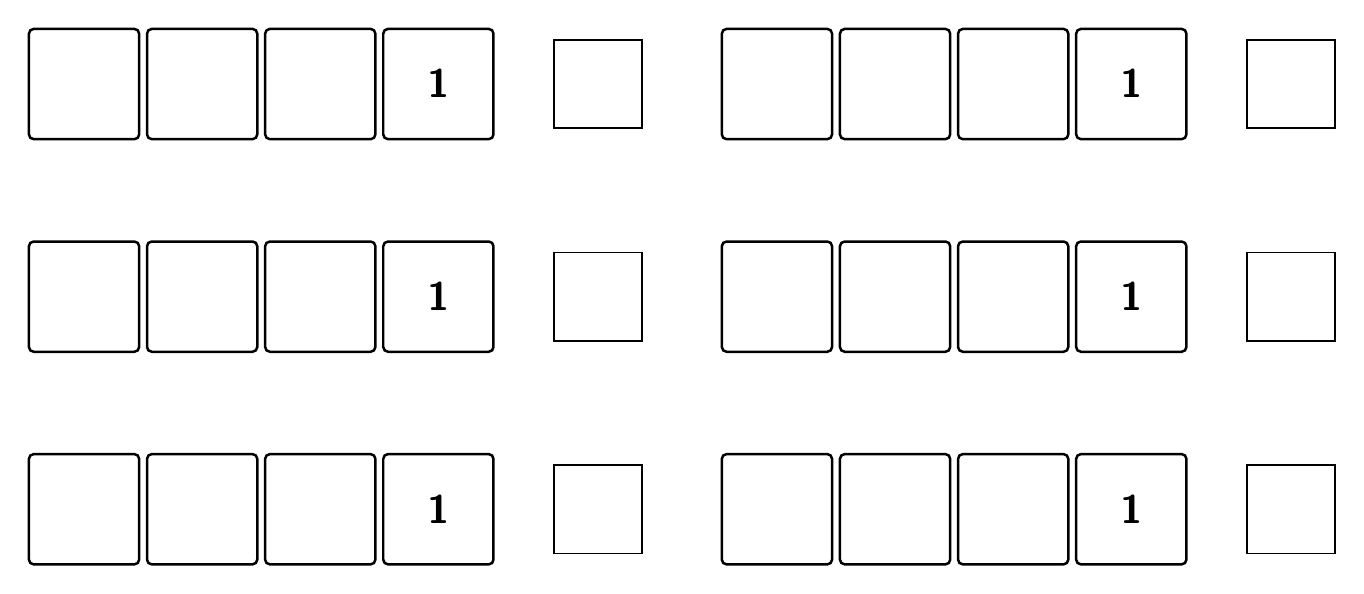
\begin{tikzpicture}[x=1mm,y=1mm]
\draw[line width=0.9pt, fill=white, rounded corners=0.6mm] (0,0) rectangle (14,14);
\draw[line width=0.9pt, fill=white, rounded corners=0.6mm] (15,0) rectangle (29,14);
\draw[line width=0.9pt, fill=white, rounded corners=0.6mm] (30,0) rectangle (44,14);
\draw[line width=0.9pt, fill=white, rounded corners=0.6mm] (45,0) rectangle (59,14);
\node at (52,7) {\bfseries\Large 1};
\draw[line width=0.6pt] (66.7,1.4) rectangle (77.9,12.6);
\draw[line width=0.9pt, fill=white, rounded corners=0.6mm] (88,0) rectangle (102,14);
\draw[line width=0.9pt, fill=white, rounded corners=0.6mm] (103,0) rectangle (117,14);
\draw[line width=0.9pt, fill=white, rounded corners=0.6mm] (118,0) rectangle (132,14);
\draw[line width=0.9pt, fill=white, rounded corners=0.6mm] (133,0) rectangle (147,14);
\node at (140,7) {\bfseries\Large 1};
\draw[line width=0.6pt] (154.7,1.4) rectangle (165.9,12.6);
\draw[line width=0.9pt, fill=white, rounded corners=0.6mm] (0,-27) rectangle (14,-13);
\draw[line width=0.9pt, fill=white, rounded corners=0.6mm] (15,-27) rectangle (29,-13);
\draw[line width=0.9pt, fill=white, rounded corners=0.6mm] (30,-27) rectangle (44,-13);
\draw[line width=0.9pt, fill=white, rounded corners=0.6mm] (45,-27) rectangle (59,-13);
\node at (52,-20) {\bfseries\Large 1};
\draw[line width=0.6pt] (66.7,-25.6) rectangle (77.9,-14.4);
\draw[line width=0.9pt, fill=white, rounded corners=0.6mm] (88,-27) rectangle (102,-13);
\draw[line width=0.9pt, fill=white, rounded corners=0.6mm] (103,-27) rectangle (117,-13);
\draw[line width=0.9pt, fill=white, rounded corners=0.6mm] (118,-27) rectangle (132,-13);
\draw[line width=0.9pt, fill=white, rounded corners=0.6mm] (133,-27) rectangle (147,-13);
\node at (140,-20) {\bfseries\Large 1};
\draw[line width=0.6pt] (154.7,-25.6) rectangle (165.9,-14.4);
\draw[line width=0.9pt, fill=white, rounded corners=0.6mm] (0,-54) rectangle (14,-40);
\draw[line width=0.9pt, fill=white, rounded corners=0.6mm] (15,-54) rectangle (29,-40);
\draw[line width=0.9pt, fill=white, rounded corners=0.6mm] (30,-54) rectangle (44,-40);
\draw[line width=0.9pt, fill=white, rounded corners=0.6mm] (45,-54) rectangle (59,-40);
\node at (52,-47) {\bfseries\Large 1};
\draw[line width=0.6pt] (66.7,-52.6) rectangle (77.9,-41.4);
\draw[line width=0.9pt, fill=white, rounded corners=0.6mm] (88,-54) rectangle (102,-40);
\draw[line width=0.9pt, fill=white, rounded corners=0.6mm] (103,-54) rectangle (117,-40);
\draw[line width=0.9pt, fill=white, rounded corners=0.6mm] (118,-54) rectangle (132,-40);
\draw[line width=0.9pt, fill=white, rounded corners=0.6mm] (133,-54) rectangle (147,-40);
\node at (140,-47) {\bfseries\Large 1};
\draw[line width=0.6pt] (154.7,-52.6) rectangle (165.9,-41.4);
\end{tikzpicture}
\end{center}

\newpage
\problem{4}Which of these trains can leave 1, 2, 3, 4, 5? Mark each one \yes{} or \no.
\par\vspace{8pt}\begin{center}
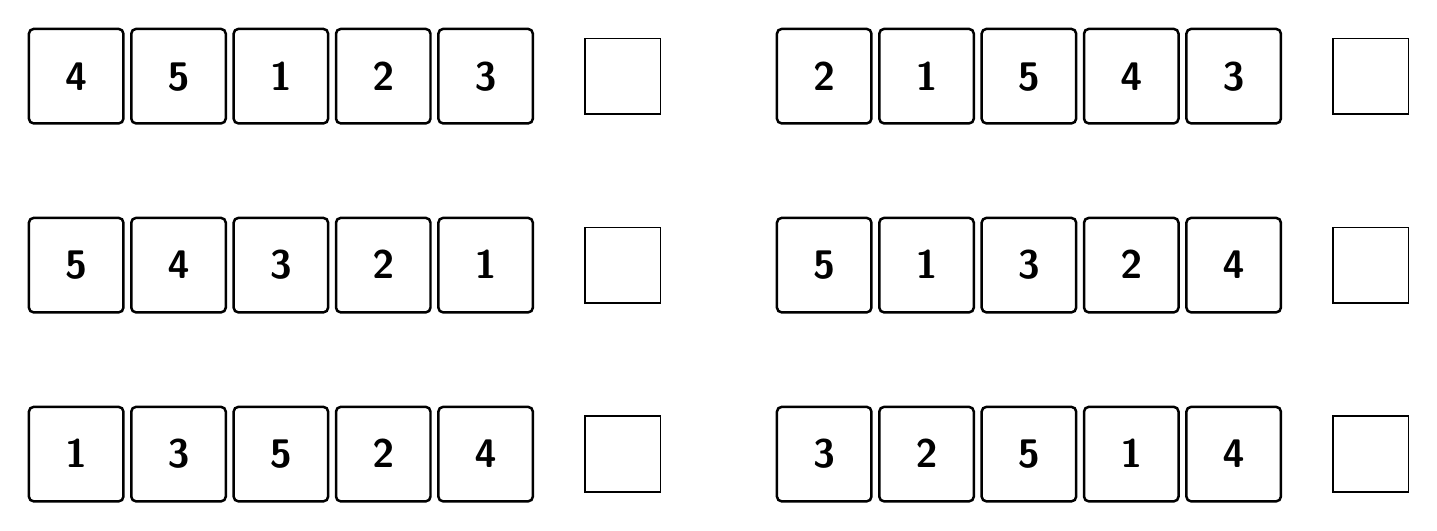
\begin{tikzpicture}[x=1mm,y=1mm]
\draw[line width=0.9pt, fill=white, rounded corners=0.6mm] (0,0) rectangle (12,12);
\node at (6,6) {\bfseries\Large 4};
\draw[line width=0.9pt, fill=white, rounded corners=0.6mm] (13,0) rectangle (25,12);
\node at (19,6) {\bfseries\Large 5};
\draw[line width=0.9pt, fill=white, rounded corners=0.6mm] (26,0) rectangle (38,12);
\node at (32,6) {\bfseries\Large 1};
\draw[line width=0.9pt, fill=white, rounded corners=0.6mm] (39,0) rectangle (51,12);
\node at (45,6) {\bfseries\Large 2};
\draw[line width=0.9pt, fill=white, rounded corners=0.6mm] (52,0) rectangle (64,12);
\node at (58,6) {\bfseries\Large 3};
\draw[line width=0.6pt] (70.6,1.2) rectangle (80.2,10.8);
\draw[line width=0.9pt, fill=white, rounded corners=0.6mm] (95,0) rectangle (107,12);
\node at (101,6) {\bfseries\Large 2};
\draw[line width=0.9pt, fill=white, rounded corners=0.6mm] (108,0) rectangle (120,12);
\node at (114,6) {\bfseries\Large 1};
\draw[line width=0.9pt, fill=white, rounded corners=0.6mm] (121,0) rectangle (133,12);
\node at (127,6) {\bfseries\Large 5};
\draw[line width=0.9pt, fill=white, rounded corners=0.6mm] (134,0) rectangle (146,12);
\node at (140,6) {\bfseries\Large 4};
\draw[line width=0.9pt, fill=white, rounded corners=0.6mm] (147,0) rectangle (159,12);
\node at (153,6) {\bfseries\Large 3};
\draw[line width=0.6pt] (165.6,1.2) rectangle (175.2,10.8);
\draw[line width=0.9pt, fill=white, rounded corners=0.6mm] (0,-24) rectangle (12,-12);
\node at (6,-18) {\bfseries\Large 5};
\draw[line width=0.9pt, fill=white, rounded corners=0.6mm] (13,-24) rectangle (25,-12);
\node at (19,-18) {\bfseries\Large 4};
\draw[line width=0.9pt, fill=white, rounded corners=0.6mm] (26,-24) rectangle (38,-12);
\node at (32,-18) {\bfseries\Large 3};
\draw[line width=0.9pt, fill=white, rounded corners=0.6mm] (39,-24) rectangle (51,-12);
\node at (45,-18) {\bfseries\Large 2};
\draw[line width=0.9pt, fill=white, rounded corners=0.6mm] (52,-24) rectangle (64,-12);
\node at (58,-18) {\bfseries\Large 1};
\draw[line width=0.6pt] (70.6,-22.8) rectangle (80.2,-13.2);
\draw[line width=0.9pt, fill=white, rounded corners=0.6mm] (95,-24) rectangle (107,-12);
\node at (101,-18) {\bfseries\Large 5};
\draw[line width=0.9pt, fill=white, rounded corners=0.6mm] (108,-24) rectangle (120,-12);
\node at (114,-18) {\bfseries\Large 1};
\draw[line width=0.9pt, fill=white, rounded corners=0.6mm] (121,-24) rectangle (133,-12);
\node at (127,-18) {\bfseries\Large 3};
\draw[line width=0.9pt, fill=white, rounded corners=0.6mm] (134,-24) rectangle (146,-12);
\node at (140,-18) {\bfseries\Large 2};
\draw[line width=0.9pt, fill=white, rounded corners=0.6mm] (147,-24) rectangle (159,-12);
\node at (153,-18) {\bfseries\Large 4};
\draw[line width=0.6pt] (165.6,-22.8) rectangle (175.2,-13.2);
\draw[line width=0.9pt, fill=white, rounded corners=0.6mm] (0,-48) rectangle (12,-36);
\node at (6,-42) {\bfseries\Large 1};
\draw[line width=0.9pt, fill=white, rounded corners=0.6mm] (13,-48) rectangle (25,-36);
\node at (19,-42) {\bfseries\Large 3};
\draw[line width=0.9pt, fill=white, rounded corners=0.6mm] (26,-48) rectangle (38,-36);
\node at (32,-42) {\bfseries\Large 5};
\draw[line width=0.9pt, fill=white, rounded corners=0.6mm] (39,-48) rectangle (51,-36);
\node at (45,-42) {\bfseries\Large 2};
\draw[line width=0.9pt, fill=white, rounded corners=0.6mm] (52,-48) rectangle (64,-36);
\node at (58,-42) {\bfseries\Large 4};
\draw[line width=0.6pt] (70.6,-46.8) rectangle (80.2,-37.2);
\draw[line width=0.9pt, fill=white, rounded corners=0.6mm] (95,-48) rectangle (107,-36);
\node at (101,-42) {\bfseries\Large 3};
\draw[line width=0.9pt, fill=white, rounded corners=0.6mm] (108,-48) rectangle (120,-36);
\node at (114,-42) {\bfseries\Large 2};
\draw[line width=0.9pt, fill=white, rounded corners=0.6mm] (121,-48) rectangle (133,-36);
\node at (127,-42) {\bfseries\Large 5};
\draw[line width=0.9pt, fill=white, rounded corners=0.6mm] (134,-48) rectangle (146,-36);
\node at (140,-42) {\bfseries\Large 1};
\draw[line width=0.9pt, fill=white, rounded corners=0.6mm] (147,-48) rectangle (159,-36);
\node at (153,-42) {\bfseries\Large 4};
\draw[line width=0.6pt] (165.6,-46.8) rectangle (175.2,-37.2);
\end{tikzpicture}
\end{center}

\vspace{6pt}
\problem{5}One partner lines up all five cars, and the other partner guesses whether they can leave 1, 2, 3, 4, 5. Drive them to check, then switch jobs.
\newpage
\problem{6}Find all 10 trains of cars 1, 2, 3, 4 that cannot leave 1, 2, 3, 4.
\par\vspace{8pt}\begin{center}
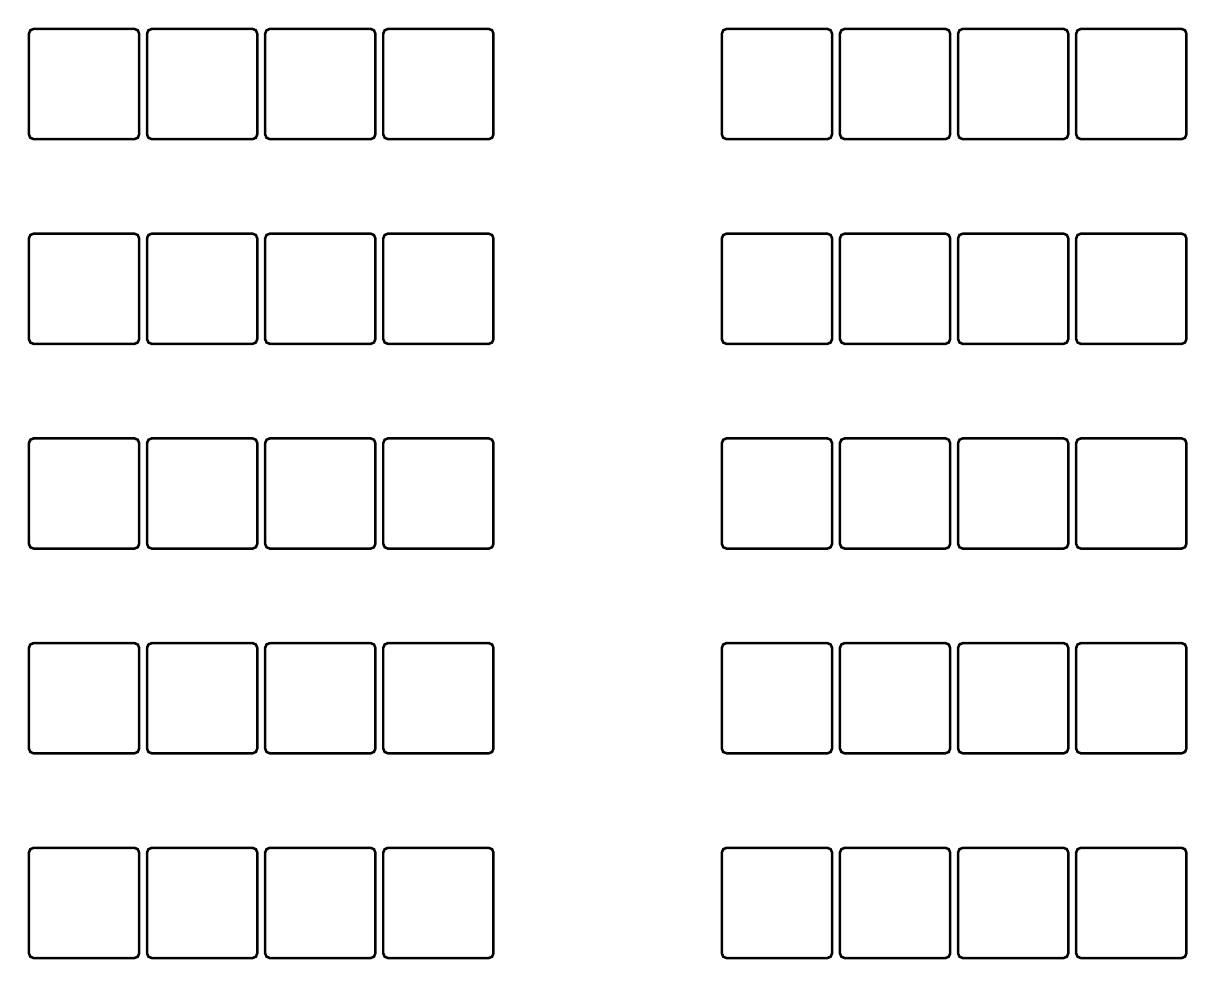
\begin{tikzpicture}[x=1mm,y=1mm]
\draw[line width=0.9pt, fill=white, rounded corners=0.6mm] (0,0) rectangle (14,14);
\draw[line width=0.9pt, fill=white, rounded corners=0.6mm] (15,0) rectangle (29,14);
\draw[line width=0.9pt, fill=white, rounded corners=0.6mm] (30,0) rectangle (44,14);
\draw[line width=0.9pt, fill=white, rounded corners=0.6mm] (45,0) rectangle (59,14);
\draw[line width=0.9pt, fill=white, rounded corners=0.6mm] (88,0) rectangle (102,14);
\draw[line width=0.9pt, fill=white, rounded corners=0.6mm] (103,0) rectangle (117,14);
\draw[line width=0.9pt, fill=white, rounded corners=0.6mm] (118,0) rectangle (132,14);
\draw[line width=0.9pt, fill=white, rounded corners=0.6mm] (133,0) rectangle (147,14);
\draw[line width=0.9pt, fill=white, rounded corners=0.6mm] (0,-26) rectangle (14,-12);
\draw[line width=0.9pt, fill=white, rounded corners=0.6mm] (15,-26) rectangle (29,-12);
\draw[line width=0.9pt, fill=white, rounded corners=0.6mm] (30,-26) rectangle (44,-12);
\draw[line width=0.9pt, fill=white, rounded corners=0.6mm] (45,-26) rectangle (59,-12);
\draw[line width=0.9pt, fill=white, rounded corners=0.6mm] (88,-26) rectangle (102,-12);
\draw[line width=0.9pt, fill=white, rounded corners=0.6mm] (103,-26) rectangle (117,-12);
\draw[line width=0.9pt, fill=white, rounded corners=0.6mm] (118,-26) rectangle (132,-12);
\draw[line width=0.9pt, fill=white, rounded corners=0.6mm] (133,-26) rectangle (147,-12);
\draw[line width=0.9pt, fill=white, rounded corners=0.6mm] (0,-52) rectangle (14,-38);
\draw[line width=0.9pt, fill=white, rounded corners=0.6mm] (15,-52) rectangle (29,-38);
\draw[line width=0.9pt, fill=white, rounded corners=0.6mm] (30,-52) rectangle (44,-38);
\draw[line width=0.9pt, fill=white, rounded corners=0.6mm] (45,-52) rectangle (59,-38);
\draw[line width=0.9pt, fill=white, rounded corners=0.6mm] (88,-52) rectangle (102,-38);
\draw[line width=0.9pt, fill=white, rounded corners=0.6mm] (103,-52) rectangle (117,-38);
\draw[line width=0.9pt, fill=white, rounded corners=0.6mm] (118,-52) rectangle (132,-38);
\draw[line width=0.9pt, fill=white, rounded corners=0.6mm] (133,-52) rectangle (147,-38);
\draw[line width=0.9pt, fill=white, rounded corners=0.6mm] (0,-78) rectangle (14,-64);
\draw[line width=0.9pt, fill=white, rounded corners=0.6mm] (15,-78) rectangle (29,-64);
\draw[line width=0.9pt, fill=white, rounded corners=0.6mm] (30,-78) rectangle (44,-64);
\draw[line width=0.9pt, fill=white, rounded corners=0.6mm] (45,-78) rectangle (59,-64);
\draw[line width=0.9pt, fill=white, rounded corners=0.6mm] (88,-78) rectangle (102,-64);
\draw[line width=0.9pt, fill=white, rounded corners=0.6mm] (103,-78) rectangle (117,-64);
\draw[line width=0.9pt, fill=white, rounded corners=0.6mm] (118,-78) rectangle (132,-64);
\draw[line width=0.9pt, fill=white, rounded corners=0.6mm] (133,-78) rectangle (147,-64);
\draw[line width=0.9pt, fill=white, rounded corners=0.6mm] (0,-104) rectangle (14,-90);
\draw[line width=0.9pt, fill=white, rounded corners=0.6mm] (15,-104) rectangle (29,-90);
\draw[line width=0.9pt, fill=white, rounded corners=0.6mm] (30,-104) rectangle (44,-90);
\draw[line width=0.9pt, fill=white, rounded corners=0.6mm] (45,-104) rectangle (59,-90);
\draw[line width=0.9pt, fill=white, rounded corners=0.6mm] (88,-104) rectangle (102,-90);
\draw[line width=0.9pt, fill=white, rounded corners=0.6mm] (103,-104) rectangle (117,-90);
\draw[line width=0.9pt, fill=white, rounded corners=0.6mm] (118,-104) rectangle (132,-90);
\draw[line width=0.9pt, fill=white, rounded corners=0.6mm] (133,-104) rectangle (147,-90);
\end{tikzpicture}
\end{center}

\end{document}
